% Created 2018-09-23 Sun 20:27
% Intended LaTeX compiler: pdflatex
\documentclass[11pt]{article}
\usepackage[utf8]{inputenc}
\usepackage{lmodern}
\usepackage[T1]{fontenc}
\usepackage{fixltx2e}
\usepackage{graphicx}
\usepackage{longtable}
\usepackage{float}
\usepackage{wrapfig}
\usepackage{rotating}
\usepackage[normalem]{ulem}
\usepackage{amsmath}
\usepackage{textcomp}
\usepackage{marvosym}
\usepackage{wasysym}
\usepackage{amssymb}
\usepackage{amsmath}
\usepackage[version=3]{mhchem}
\usepackage[numbers,super,sort&compress]{natbib}
\usepackage{natmove}
\usepackage{url}
\usepackage{minted}
\usepackage{underscore}
\usepackage[linktocpage,pdfstartview=FitH,colorlinks,
linkcolor=blue,anchorcolor=blue,
citecolor=blue,filecolor=blue,menucolor=blue,urlcolor=blue]{hyperref}
\usepackage{attachfile}
\author{Myrthe Boone}
\date{\today}
\title{Predicting survival on the Titanic}
\begin{document}

\tableofcontents

In this paper we look at the chances of surviving the Titanic using
python. We predict the chances of an unseen set of data by using
supervised machinelearning on the known dataset.

We use information from \href{http://www.encyclopedia-titanica.org}{this
site}.

This is one of the first drafts to get to know the dataset and to
experiment with the python and all the packages included.


\section{Preparation}
\label{preparation}
\begin{minted}[frame=lines,fontsize=\scriptsize,linenos]{ipython}
    import numpy as np
    import pandas as pd
    import matplotlib.pyplot as plt
    import seaborn as sns
\end{minted}

The adventure begins with importing the right packages. The dataset is
downloaded from \href{https://www.kaggle.com/c/titanic/data}{kaggle site}
as csv$\backslash$\_file. Next the data is read into a dataframe by using pandas'
pd.read$\backslash$\_csv

\begin{minted}[frame=lines,fontsize=\scriptsize,linenos]{ipython}
    data = pd.read_csv('titanic.csv')
\end{minted}

Here we see the head of our dataframe. A couple of questions come to
mind. Which variables play a role by determining the probability of
surviving the Titanic. Sex and Cabin are not numeric values. How do we
convert these to numeric values?

\section{A first look at the dataset}
\label{a-first-look-at-the-dataset}
\begin{minted}[frame=lines,fontsize=\scriptsize,linenos]{ipython}
    data.head()
\end{minted}

\begin{verbatim}
   PassengerId  Survived  Pclass  \
0            1         0       3   
1            2         1       1   
2            3         1       3   
3            4         1       1   
4            5         0       3   

                                                Name     Sex   Age  SibSp  \
0                            Braund, Mr. Owen Harris    male  22.0      1   
1  Cumings, Mrs. John Bradley (Florence Briggs Th...  female  38.0      1   
2                             Heikkinen, Miss. Laina  female  26.0      0   
3       Futrelle, Mrs. Jacques Heath (Lily May Peel)  female  35.0      1   
4                           Allen, Mr. William Henry    male  35.0      0   

   Parch            Ticket     Fare Cabin Embarked  
0      0         A/5 21171   7.2500   NaN        S  
1      0          PC 17599  71.2833   C85        C  
2      0  STON/O2. 3101282   7.9250   NaN        S  
3      0            113803  53.1000  C123        S  
4      0            373450   8.0500   NaN        S  
\end{verbatim}

Here are the summary statistics of the dataframe. The mean,
standarddeviation etc are given in this table.

\begin{minted}[frame=lines,fontsize=\scriptsize,linenos]{ipython}
    data.describe()
\end{minted}

\begin{verbatim}
       PassengerId    Survived      Pclass         Age       SibSp  \
count   891.000000  891.000000  891.000000  714.000000  891.000000   
mean    446.000000    0.383838    2.308642   29.699118    0.523008   
std     257.353842    0.486592    0.836071   14.526497    1.102743   
min       1.000000    0.000000    1.000000    0.420000    0.000000   
25%     223.500000    0.000000    2.000000   20.125000    0.000000   
50%     446.000000    0.000000    3.000000   28.000000    0.000000   
75%     668.500000    1.000000    3.000000   38.000000    1.000000   
max     891.000000    1.000000    3.000000   80.000000    8.000000   

            Parch        Fare  
count  891.000000  891.000000  
mean     0.381594   32.204208  
std      0.806057   49.693429  
min      0.000000    0.000000  
25%      0.000000    7.910400  
50%      0.000000   14.454200  
75%      0.000000   31.000000  
max      6.000000  512.329200  
\end{verbatim}

It is possible to search for particular passenger in the dataset. Such
as passengers who were older than eighty years.

\begin{minted}[frame=lines,fontsize=\scriptsize,linenos]{ipython}
    data[data.Age == 80]
\end{minted}

\begin{verbatim}
     PassengerId  Survived  Pclass                                  Name  \
630          631         1       1  Barkworth, Mr. Algernon Henry Wilson   

      Sex   Age  SibSp  Parch Ticket  Fare Cabin Embarked  
630  male  80.0      0      0  27042  30.0   A23        S  
\end{verbatim}

\section{First figures}
\label{first-figures}
To get a good impression of the dataset and the influence of the
variables, a couple of diagrams are made using \texttt{mathplotlib}.

\begin{minted}[frame=lines,fontsize=\scriptsize,linenos]{ipython}
    plt.scatter(data.Age,data.Survived)
    plt.xlabel('Age')
    plt.ylabel('Survived')
\end{minted}

\begin{verbatim}
Text(0,0.5,'Survived')
\end{verbatim}



\begin{center}
\includegraphics[width=.9\linewidth]{obipy-resources/37cee3acc6d688dc7952727caad1e09e-1377maP.png}
\end{center}


Scatterplots are not always the best choice to illustrate some of the
variables. There is not much to say about the variance because of the
fact that a lot of points are close to eachother. A couple of values
however stand out. We see that a passenger or more passengers travelling
first class have paid more than 500 pounds for their ticketprice.

\begin{minted}[frame=lines,fontsize=\scriptsize,linenos]{ipython}
    plt.scatter(data.Pclass,data.Fare)
    plt.xlabel('Pclass')
    plt.ylabel('Fare')
\end{minted}

\begin{verbatim}
Text(0,0.5,'Fare')
\end{verbatim}



\begin{center}
\includegraphics[width=.9\linewidth]{obipy-resources/37cee3acc6d688dc7952727caad1e09e-1377zkV.png}
\end{center}

\begin{minted}[frame=lines,fontsize=\scriptsize,linenos]{ipython}
    plt.scatter(data.Fare, data.Survived)
    plt.xlabel('Fare')
    plt.ylabel('Survived')
\end{minted}

\begin{verbatim}
Text(0,0.5,'Survived')
\end{verbatim}



\begin{center}
\includegraphics[width=.9\linewidth]{obipy-resources/37cee3acc6d688dc7952727caad1e09e-1377Avb.png}
\end{center}

\begin{minted}[frame=lines,fontsize=\scriptsize,linenos]{ipython}
    plt.scatter(data.Fare, data.Age)
    plt.xlabel('Fare')
    plt.ylabel('Age')
\end{minted}

\begin{verbatim}
Text(0,0.5,'Age')
\end{verbatim}



\begin{center}
\includegraphics[width=.9\linewidth]{obipy-resources/37cee3acc6d688dc7952727caad1e09e-1377N5h.png}
\end{center}

I was curious to see who had paid more than 400 pounds for their ticket.
We see that it is easy to make a selection in our dataset using the \texttt{>}
sign

\begin{minted}[frame=lines,fontsize=\scriptsize,linenos]{ipython}
    data[data.Fare > 400]
\end{minted}

\begin{verbatim}
     PassengerId  Survived  Pclass                                Name  \
258          259         1       1                    Ward, Miss. Anna   
679          680         1       1  Cardeza, Mr. Thomas Drake Martinez   
737          738         1       1              Lesurer, Mr. Gustave J   

        Sex   Age  SibSp  Parch    Ticket      Fare        Cabin Embarked  
258  female  35.0      0      0  PC 17755  512.3292          NaN        C  
679    male  36.0      0      1  PC 17755  512.3292  B51 B53 B55        C  
737    male  35.0      0      0  PC 17755  512.3292         B101        C  
\end{verbatim}

\begin{minted}[frame=lines,fontsize=\scriptsize,linenos]{ipython}
    df_cleaned = data.dropna()
    df_cleaned['male_dummy'] = (df_cleaned.Sex == 'male') #nieuwe kolom definiëren om male te veranderen in een boolean
    X = df_cleaned[['Age','male_dummy', 'Pclass', 'SibSp', 'Fare']]
    y = df_cleaned[['Survived']]
\end{minted}

\begin{verbatim}
/Users/myrthe/anaconda3/lib/python3.6/site-packages/ipykernel_launcher.py:2: SettingWithCopyWarning: 
A value is trying to be set on a copy of a slice from a DataFrame.
Try using .loc[row_indexer,col_indexer] = value instead

See the caveats in the documentation: http://pandas.pydata.org/pandas-docs/stable/indexing.html#indexing-view-versus-copy
  

\end{verbatim}

Here we see that we clean our dataset for the first time to make it more
suitable for the packages we will be using. All rows with missing values
(these are called NaNs, short for Not a Number) are deleted for
scikit$\backslash$\_learn can't work with NaNs by using \texttt{.dropna()}. There are other
ways than deleting rows to handle this problem. Replace the NaNs with
the mean or to interpolate for example. However the choice was made to
delete these rows. Furthermore we see that the problem of the \texttt{Sex}
column not being a numeric value is handled. The values in the \texttt{Sex}
column are changed into a boolean. Males are given a \texttt{True} and the
females are given a \texttt{False}. Next a couple of variables have added to
\texttt{X}. \texttt{Age},=male\_dummy=, \texttt{Pclass}, \texttt{SibSp}, \texttt{Fare} are all numeric
values and therefore easy to use.

Here we see the cleaned dataframe with the new added column \texttt{male\_dummy}

\begin{minted}[frame=lines,fontsize=\scriptsize,linenos]{ipython}
    df_cleaned.head()
\end{minted}

\begin{verbatim}
    PassengerId  Survived  Pclass  \
1             2         1       1   
3             4         1       1   
6             7         0       1   
10           11         1       3   
11           12         1       1   

                                                 Name     Sex   Age  SibSp  \
1   Cumings, Mrs. John Bradley (Florence Briggs Th...  female  38.0      1   
3        Futrelle, Mrs. Jacques Heath (Lily May Peel)  female  35.0      1   
6                             McCarthy, Mr. Timothy J    male  54.0      0   
10                    Sandstrom, Miss. Marguerite Rut  female   4.0      1   
11                           Bonnell, Miss. Elizabeth  female  58.0      0   

    Parch    Ticket     Fare Cabin Embarked  male_dummy  
1       0  PC 17599  71.2833   C85        C       False  
3       0    113803  53.1000  C123        S       False  
6       0     17463  51.8625   E46        S        True  
10      1   PP 9549  16.7000    G6        S       False  
11      0    113783  26.5500  C103        S       False  
\end{verbatim}

\begin{minted}[frame=lines,fontsize=\scriptsize,linenos]{ipython}
    from sklearn.linear_model import LogisticRegression
    logreg = LogisticRegression()
    logreg.fit(X, y)
    y_pred = logreg.predict(X)
\end{minted}

\begin{verbatim}
/Users/myrthe/anaconda3/lib/python3.6/site-packages/sklearn/utils/validation.py:578: DataConversionWarning: A column-vector y was passed when a 1d array was expected. Please change the shape of y to (n_samples, ), for example using ravel().
  y = column_or_1d(y, warn=True)

\end{verbatim}

Here we initialize the first regression called logistic regression. We
don't split our dataframe in test and training set yet. For a general
indication we only use the regressor and fit it on the cleaned dataset.
After that we predict on the same dataset.

\begin{minted}[frame=lines,fontsize=\scriptsize,linenos]{ipython}
    logreg.coef_
\end{minted}

\begin{verbatim}
array([[-0.01636209, -2.08109476,  0.01318695,  0.2035389 ,  0.00296447]])
\end{verbatim}

Here we see the outcome of our first try with the logistic regression.

To interpret these coefficients, let's look at the order of the columns
in \texttt{X}:

\begin{minted}[frame=lines,fontsize=\scriptsize,linenos]{ipython}
    X.head()
\end{minted}

\begin{verbatim}
     Age  male_dummy  Pclass  SibSp     Fare
1   38.0       False       1      1  71.2833
3   35.0       False       1      1  53.1000
6   54.0        True       1      0  51.8625
10   4.0       False       3      1  16.7000
11  58.0       False       1      0  26.5500
\end{verbatim}

\section{Graphic illustration of a prediction}
\label{graphic-illustration-of-a-prediction}
One of the first graphic illustrations of the relation between fare, age
and survival. The relation is not very clear but we see that the higher
the fare the more people survived and the higher the age the less people
survived. However, this figure is not very accurate, because of the fact
that only three variables were used.

\begin{minted}[frame=lines,fontsize=\scriptsize,linenos]{ipython}
    survived = df_cleaned[df_cleaned.Survived == 1]
    not_survived = df_cleaned[df_cleaned.Survived == 0]

    plt.scatter(survived.Fare, survived.Age, marker='^', label = 'survived')
    plt.scatter(not_survived.Fare, not_survived.Age, marker='^', label = 'not survived')
    plt.legend()
\end{minted}

\begin{center}
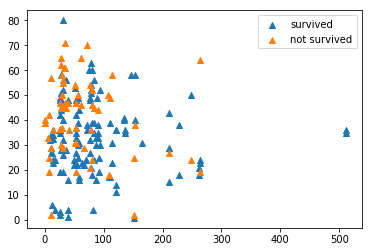
\includegraphics[width=.9\linewidth]{obipy-resources/37cee3acc6d688dc7952727caad1e09e-1377aDo.png}
\end{center}

\begin{minted}[frame=lines,fontsize=\scriptsize,linenos]{ipython}
    P = df_cleaned[['Pclass', 'Fare','Age','male_dummy']]
\end{minted}

We select from our df$\backslash$\_cleaned only the columns with numeric values.
This is convenient for the splitting into train and testsets, for
scikit$\backslash$\_learn can only work with numbers. Difference between P and X
here is that X also has the column siblings, whereas P only has four
columns

\begin{minted}[frame=lines,fontsize=\scriptsize,linenos]{ipython}
    P.head()
\end{minted}

\begin{verbatim}
    Pclass     Fare   Age  male_dummy
1        1  71.2833  38.0       False
3        1  53.1000  35.0       False
6        1  51.8625  54.0        True
10       3  16.7000   4.0       False
11       1  26.5500  58.0       False
\end{verbatim}

\begin{HTML}
<div>
<style scoped>
    .dataframe tbody tr th:only-of-type \{
	vertical-align: middle;
    \}

.dataframe tbody tr th \{
    vertical-align: top;
\}

    .dataframe thead th \{
	text-align: right;
    \}
</style>
<table border="1" class="dataframe">
  <thead>
    <tr style="text-align: right;">
      <th></th>
      <th>Pclass</th>
      <th>Fare</th>
      <th>Age</th>
      <th>male\_dummy</th>
    </tr>
  </thead>
  <tbody>
    <tr>
      <th>1</th>
      <td>1</td>
      <td>71.2833</td>
      <td>38.0</td>
      <td>False</td>
    </tr>
    <tr>
      <th>3</th>
      <td>1</td>
      <td>53.1000</td>
      <td>35.0</td>
      <td>False</td>
    </tr>
    <tr>
      <th>6</th>
      <td>1</td>
      <td>51.8625</td>
      <td>54.0</td>
      <td>True</td>
    </tr>
    <tr>
      <th>10</th>
      <td>3</td>
      <td>16.7000</td>
      <td>4.0</td>
      <td>False</td>
    </tr>
    <tr>
      <th>11</th>
      <td>1</td>
      <td>26.5500</td>
      <td>58.0</td>
      <td>False</td>
    </tr>
  </tbody>
</table>
</div>
\end{HTML}

\begin{minted}[frame=lines,fontsize=\scriptsize,linenos]{ipython}
    from sklearn.linear_model import LogisticRegression
    logreg = LogisticRegression(fit_intercept=True)
    logreg.fit(P, y)
    y_pred = logreg.predict(P)
\end{minted}

\begin{verbatim}
/Users/myrthe/anaconda3/lib/python3.6/site-packages/sklearn/utils/validation.py:578: DataConversionWarning: A column-vector y was passed when a 1d array was expected. Please change the shape of y to (n_samples, ), for example using ravel().
  y = column_or_1d(y, warn=True)

\end{verbatim}

We fit our regressor on our dataset and predict on that same dataset.
Once again without splitting into train and testset. Just to get a
general idea about the values of the coeffecients.

\begin{minted}[frame=lines,fontsize=\scriptsize,linenos]{ipython}
    logreg.coef_
\end{minted}

\begin{verbatim}
array([[ 0.00917324,  0.00337838, -0.01693475, -2.07643966]])
\end{verbatim}

One could interpret the found coeffecients as follows: The coeffecients
for class and fare are positive, which may indicate that the higher the
class and price paid for a ticket, the higher the chance of surviving
the Titanic. When we look at age and sex we see the exact opposite for
the coeffecients are negative. The higher the age the lower your chances
and if you were a man on board of the titanic your chances of surviving
were lower.

\begin{minted}[frame=lines,fontsize=\scriptsize,linenos]{ipython}
    from sklearn.neighbors import KNeighborsClassifier
\end{minted}

Another regression is used in the following lines. (explanation K
nearest neighbours)

\begin{minted}[frame=lines,fontsize=\scriptsize,linenos]{ipython}
    knn = KNeighborsClassifier(n_neighbors=6)
\end{minted}

\begin{minted}[frame=lines,fontsize=\scriptsize,linenos]{ipython}
    knn.fit(P,y)
\end{minted}

\begin{verbatim}
/Users/myrthe/anaconda3/lib/python3.6/site-packages/ipykernel_launcher.py:1: DataConversionWarning: A column-vector y was passed when a 1d array was expected. Please change the shape of y to (n_samples, ), for example using ravel().
  """Entry point for launching an IPython kernel.

\end{verbatim}

\begin{verbatim}
KNeighborsClassifier(algorithm='auto', leaf_size=30, metric='minkowski',
           metric_params=None, n_jobs=1, n_neighbors=6, p=2,
           weights='uniform')
\end{verbatim}

\begin{minted}[frame=lines,fontsize=\scriptsize,linenos]{ipython}
    prediction = knn.predict(P)
\end{minted}

\begin{minted}[frame=lines,fontsize=\scriptsize,linenos]{ipython}
    P.shape
\end{minted}

\begin{verbatim}
(183, 4)
\end{verbatim}

\begin{minted}[frame=lines,fontsize=\scriptsize,linenos]{ipython}
    print('Prediction{}'.format(prediction))
\end{minted}

\begin{verbatim}
Prediction[1 0 0 1 0 1 1 1 1 0 0 1 1 1 1 0 1 1 1 1 1 1 1 1 1 1 1 0 0 1 1 1 0 1 1 1 1
 1 1 1 1 1 1 0 1 1 0 1 1 1 1 1 1 1 1 1 1 1 1 1 1 1 1 1 1 0 1 1 1 0 1 1 1 1
 1 1 1 1 1 1 1 1 1 1 1 1 1 1 0 1 0 0 1 0 1 1 1 0 0 1 1 1 1 1 0 1 1 1 0 1 1
 0 1 0 0 0 1 1 1 0 1 1 1 1 1 1 1 0 1 0 0 1 1 0 0 0 1 1 1 1 1 0 0 1 1 0 1 1
 1 1 1 1 1 1 1 1 0 1 1 1 1 1 0 1 1 1 0 1 1 0 0 0 1 1 1 1 1 1 1 0 1 1 1]

\end{verbatim}

Here we see one of our first predictions. 1 indicates the passenger has
survived and 0 indicates that the passenger has died

Elke persoon heeft andere karakteristieken, dus dit zijn voorspellingen
per persoon. Dus er komt een kans uit en dan kijkt de regressor, boven
of onder 0.5

\begin{minted}[frame=lines,fontsize=\scriptsize,linenos]{ipython}
    knn.score(P,y)
\end{minted}

\begin{verbatim}
0.7486338797814208
\end{verbatim}

This score gives a number between 0 and 1 and gives an impression of the
accuracy of our model. However, this accuracy is not an indication of
how well our model performs (explanation spam mail etc.)

\begin{minted}[frame=lines,fontsize=\scriptsize,linenos]{ipython}
    P.head()
\end{minted}

\begin{verbatim}
    Pclass     Fare   Age  male_dummy
1        1  71.2833  38.0       False
3        1  53.1000  35.0       False
6        1  51.8625  54.0        True
10       3  16.7000   4.0       False
11       1  26.5500  58.0       False
\end{verbatim}

\begin{minted}[frame=lines,fontsize=\scriptsize,linenos]{ipython}
    q = df_cleaned.Survived
\end{minted}

\begin{minted}[frame=lines,fontsize=\scriptsize,linenos]{ipython}
    q.head()
\end{minted}

\begin{verbatim}
1     1
3     1
6     0
10    1
11    1
Name: Survived, dtype: int64
\end{verbatim}

\begin{minted}[frame=lines,fontsize=\scriptsize,linenos]{ipython}
    from sklearn.linear_model import LogisticRegression
\end{minted}

\begin{minted}[frame=lines,fontsize=\scriptsize,linenos]{ipython}
    from sklearn.model_selection import train_test_split
\end{minted}

\begin{minted}[frame=lines,fontsize=\scriptsize,linenos]{ipython}
    logreg = LogisticRegression()
    P_train, P_test, q_train, q_test = train_test_split(P,q, test_size=0.2, random_state=42)
    logreg.fit(P_train, q_train)
    q_pred = logreg.predict(P_test)
\end{minted}

Here we see the dataset being split into a test and a training set. The
arguments give us information about how much of our data we use as a
test$\backslash$\_set and how much of our data we use as a training$\backslash$\_set. This and
the parameters will be varied to see which parameter gives the best
prediction. We fit our regressor on the training$\backslash$\_set and predict on the
test$\backslash$\_set.

\begin{minted}[frame=lines,fontsize=\scriptsize,linenos]{ipython}
    print('Prediction {}'.format(q_pred))
\end{minted}

\begin{verbatim}
Prediction [1 1 1 0 0 0 1 1 1 0 0 1 0 1 0 0 1 0 0 1 1 1 0 1 0 1 1 0 1 1 1 1 0 1 1 1 1]

\end{verbatim}

\begin{minted}[frame=lines,fontsize=\scriptsize,linenos]{ipython}
    P_train.head()
\end{minted}

\begin{verbatim}
     Pclass     Fare   Age  male_dummy
331       1  28.5000  45.5        True
336       1  66.6000  29.0        True
193       2  26.0000   3.0        True
75        3   7.6500  25.0        True
248       1  52.5542  37.0        True
\end{verbatim}

\begin{minted}[frame=lines,fontsize=\scriptsize,linenos]{ipython}
    from sklearn.metrics import roc_auc_score
    q_pred_prob = logreg.predict_proba(P_test)[:,1]
    roc_auc_score(q_test, q_pred_prob)
\end{minted}

\begin{verbatim}
0.8416149068322981
\end{verbatim}

When the test$\backslash$\_size is changed from 0.4 to 0.2 , the score increases
with more than 10\%. This makes sense because a smaller test$\backslash$\_set gives a
higher accuracy score.

\begin{minted}[frame=lines,fontsize=\scriptsize,linenos]{ipython}
    from sklearn.model_selection import cross_val_score
    cv_scores = cross_val_score(logreg, P, q, cv=5, scoring='roc_auc')
    print(cv_scores)
\end{minted}

\begin{verbatim}
[0.86666667 0.80333333 0.74666667 0.73263889 0.92361111]

\end{verbatim}

\begin{minted}[frame=lines,fontsize=\scriptsize,linenos]{ipython}
    len(P)
\end{minted}

\begin{verbatim}
183
\end{verbatim}

\begin{minted}[frame=lines,fontsize=\scriptsize,linenos]{ipython}
    len(prediction)
\end{minted}

\begin{verbatim}
183
\end{verbatim}

Seaborn countplot option? plt.figure()

sns.countplot(x='education', hue='party', data=df, palette='RdBu')

plt.xticks([0,1], ['No', 'Yes']) plt.show()

Given all the variables (age, gender, place of boarding etc.), you make
a linear function (a1x1+a2x2+anxn+b). Computer puts this in the logistic
function for x. For a particular x, you get a value between zero and
one. This is your chance of survival. Boundary is 0,5. X < 0,5 passenger
didn't survive. Computer tries to plot a logistic function where R2 is
as small as possible. This is called the fitting process. The logistic
function has to be as close to the datapoints as possible.

\begin{minted}[frame=lines,fontsize=\scriptsize,linenos]{ipython}
    sns.countplot?
\end{minted}

\begin{minted}[frame=lines,fontsize=\scriptsize,linenos]{ipython}
    sns.set(style="darkgrid")
    ax = sns.countplot(x="Pclass",hue="Survived", data=data, palette="Set3")
\end{minted}

\begin{center}
\includegraphics[width=.9\linewidth]{obipy-resources/37cee3acc6d688dc7952727caad1e09e-1377nNu.png}
\end{center}

More people in class 3 than in class 1, makes it difficult to compare
and draw a conclusion. Percentage? In general, we cannot draw a
conclusion regarding survival probabilities because there were more
people in class 3 than in one 1. In the third class, more passengers
died than survived. In the first class, more people survived than
perished. We cannot compare the results from the first class to the
third class. The plot only shows us one variable. This is another reason
why we cannot be sure about the influence of class on the chance of
survival. \emph{Simpson paradox}

\begin{minted}[frame=lines,fontsize=\scriptsize,linenos]{ipython}
    sns.set(style="darkgrid")
    ax = sns.countplot(x="Age",hue="Survived", data=data, palette="Set1")
\end{minted}

\begin{center}
\includegraphics[width=.9\linewidth]{obipy-resources/37cee3acc6d688dc7952727caad1e09e-13770X0.png}
\end{center}

\begin{minted}[frame=lines,fontsize=\scriptsize,linenos]{ipython}
    sns.set(style="darkgrid")
    ax = sns.countplot(x="Fare",hue="Survived", data=data)
\end{minted}

\begin{center}
\includegraphics[width=.9\linewidth]{obipy-resources/37cee3acc6d688dc7952727caad1e09e-1377mhD.png}
\end{center}

\begin{minted}[frame=lines,fontsize=\scriptsize,linenos]{ipython}
    sns.set(style="darkgrid")
    ax = sns.countplot(x="male_dummy",hue="Survived", data=df_cleaned, palette="Set2")
\end{minted}

\begin{center}
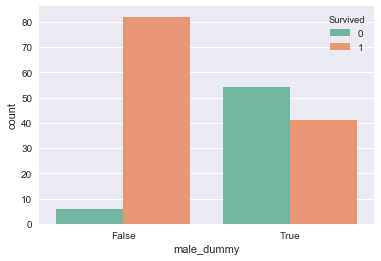
\includegraphics[width=.9\linewidth]{obipy-resources/37cee3acc6d688dc7952727caad1e09e-1377zrJ.png}
\end{center}
\end{document}